\clearpage \newpage
\subsection{Experimentos}

A continuación se presentara una breve explicación de los elementos que compusieron los experimentos, se realizaron 15 experimentos con los problemas de TSP de la fuente\cite{[TSPLIB]} por la Universidad de Heidelberg, se hicieron 100 corridas de cada problema con el fin de obtener diferentes resultados, todos los experimentos mantienen la misma configuración y se prefirió no ajustarla con el fin de asegurar el mismo rendimiento en ambos problemas.\\
Como se puede observar en la figura \ref {fig:ExplicacionExperimento.png} los datos arrojados quedaron registrados en las siguientes 3 presentaciones:

\begin{enumerate}[label=\Alph*.-]
\item Una tabla comparativa del mismo experimento, donde se muestra los resultados agrupados por tipo de metaheuristica y si se aplico o no el método de cuadrantes, las celdas coloreadas en ayuda a representar entre los 3 el mejor resultado, el mejor porcentaje y de los peores resultados el que tuvo un resultado mas pequeño.
\item Una imagen comparativa del resultado original (sin aplicar metaheuristicas) y otros que muestra aplicando el mejor resultado (en ambos están aplicando cuadrantes).
\item Una gráfica comparativa mostrando los resultados de las 100 corridas, ordenados de manera descendente para observar el progreso comparado con las demás metaheuristicas esta dividido si el problema fue resuelto por la aplicación o no de el método de cuadrantes.
\end{enumerate}

\clearpage \newpage

\begin{figure}[hbtp]
    \centering
        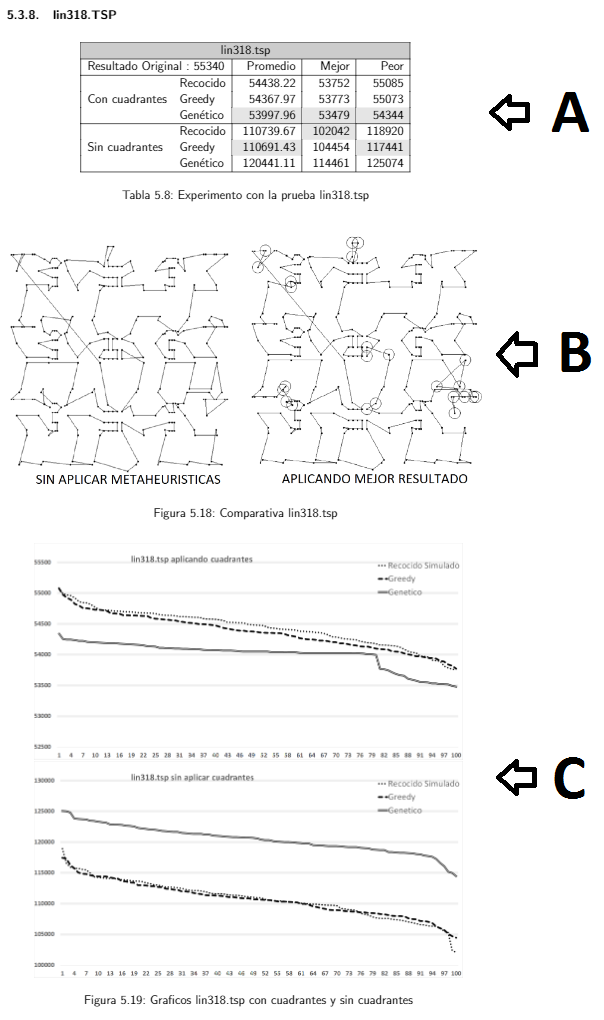
\includegraphics[width=0.6\textwidth]{PruebasResultados/Imagenes/ExplicacionExperimento.png}
        \caption{Explicación Experimento}
        \label{fig:ExplicacionExperimento.png}
\end{figure}
\clearpage \newpage

\begin{lstlisting}[language=C++, caption=Algoritmo Recocido Simulado aplicado en las pruebas, label=lst:AlgoritmoRecocidoSimuladoPruebas]
Inicio

Ciclos /*Cantidad de veces que se repetirá el proceso*/
Genes máximos /*La cantidad de genes que tendrá la especie durante el proceso de búsqueda local*/
Distancia gen mínimo /*El numero mínimo que tendrá en el intercambio de posiciones*/
Distancia gen máximo /*El numero máximo que tendrá en el intercambio de posiciones*/
Factor de temperatura /*Valor que ira alterandose durante el proceso de recocido simulado (este valor es multiplicado internamente por 1x10n12)*/

Recibir una lista de puntos para trabajar convirtiéndose en la lista de puntos actual.
MIENTRAS(NO se hayan cumplido la cantidad de Ciclos){
	1.- Crear una nueva especie con una longitud igual a la cantidad de genes máximos.
	2.- Los números que conformara la especie oscilara entre el numero mínimo y máximo declarados anteriormente.
	3.- Una vez declarada alterara la lista de puntos actual para obtener una lista nueva.
	4.- Una vez alterada la lista de puntos actual con la nueva, en caso de obtener un mejor resultado 
	SI(el resultado es mejor){
		1.-esta lista es sustituida por la nueva.
	}SINO{
		1.-Aplicar formula de temperatura
		SI(APLICA){
		    1.-La especie, aunque ineficiente se convierte en la lista de puntos actual.
		    2.-Se ajusta la temperatura.
		}
	}
}
Fin;
\end{lstlisting}

\begin{table}[hbtp]
 \centering 
  \small
   \setlength{\parskip}{1mm}
	\begin{tabular}{ | l | r | }
        \hline\multicolumn{2}{|c|}{ \rowcolor[gray]{0.75}Recocido Simulado} \\\hline
			\cellcolor[gray]{0.9}Ciclos & 10000 \\\hline
			\cellcolor[gray]{0.9}Factor temperatura & 600 \\\hline
    		\cellcolor[gray]{0.9}Genes máximos & 100 \\\hline
			\cellcolor[gray]{0.9}Distancia Gen mínimo & 2 \\\hline
			\cellcolor[gray]{0.9}Distancia Gen máximo & 5 \\\hline
    \end{tabular}
    \caption{Configuración de las variables de Recocido simulado durante las pruebas}
    \label{table:ConfiguracionRS.tsp}
\end{table}


\begin{lstlisting}[language=C++, caption=Algoritmo Greedy aplicado en las pruebas, label=lst:AlgoritmoGreedyPruebas]
Inicio

Ciclos /*Cantidad de veces que se repetirá el proceso*/
Genes máximos /*La cantidad de genes que tendrá la especie durante el proceso de búsqueda local*/
Distancia gen mínimo /*El numero mínimo que tendrá en el intercambio de posiciones*/
Distancia gen máximo /*El numero máximo que tendrá en el intercambio de posiciones*/

Recibir una lista de puntos para trabajar convirtiéndose en la lista de puntos actual.
MIENTRAS(NO se hayan cumplido la cantidad de Ciclos){
	1.- Crear una nueva especie con una longitud igual a la cantidad de genes máximos
	2.- Los números que conformara la especie oscilara entre el numero mínimo y máximo declarados anteriormente
	3.- Una vez declarada alterara la lista de puntos actual para obtener una lista nueva.
	4.- Una vez alterada la lista de puntos actual con la nueva, en caso de obtener un mejor resultado esta lista es sustituida por la nueva
}

Fin;
\end{lstlisting}

\begin{table}[hbtp]
 \centering 
  \small
	\begin{tabular}{ | l | r |}

	    \multicolumn{2}{|c|}{ \rowcolor[gray]{0.75}Greedy} \\\hline
			\cellcolor[gray]{0.9}Ciclos & 10000 \\\hline
			\cellcolor[gray]{0.9}Genes máximos & 100 \\\hline
			\cellcolor[gray]{0.9}Distancia Gen mínimo & 2 \\\hline
			\cellcolor[gray]{0.9}Distancia Gen máximo & 5 \\\hline
    \end{tabular}
    \caption{Configuración de las variables de método Greedy durante las pruebas}
    \label{table:ConfiguracionGR.tsp}
\end{table}

\begin{lstlisting}[language=C++, caption=Algoritmo Genetico aplicado en las pruebas, label=lst:AlgoritmoGeneticoPruebas]
Inicio

Generaciones /*Cantidad de veces que se repetira el proceso, en este caso la cantidad de nuevas generaciones de hijos*/
Poblacion /*Cantidad maxima que tendra cada generacion, en caso de ser impar se eliminara el unico que quede sin pareja durante el proceso de cruza*/
Genes máximos /*La cantidad de genes que tendrá la especie durante el proceso de búsqueda local*/
Distancia gen mínimo /*El numero mínimo que tendrá en el intercambio de posiciones*/
Distancia gen máximo /*El numero máximo que tendrá en el intercambio de posiciones*/
Rango de mutación mínimo /*Valor aleatorio mínimo de genes que seran modificados durante la mutacion, esta cantidad es un porcentaje se calcula con el valor de genes maximos*/
Rango de mutación máximo /*Valor aleatorio máximo de genes que seran modificados durante la mutacion, esta cantidad es un porcentaje se calcula con el valor de genes maximos*/

1.-Recibir una lista de puntos para trabajar convirtiendose en la lista de puntos actual.
MIENTRAS(NO se hayan creado la cantidad de Generaciones establecidas){
	1.-Se crea una nueva poblacion conformada de Especies.
	2.-Cada Especie tiene una cantidad de genes igual al valor de genes maximos y sus valores oscilan entre los numeros maximos y minimos de distancia.
	3.-Todas las especies se cruzan con la lista de puntos actual, se ordenan de acuerdo a su desempeño.
	4.-Si mejor especie supera a la solucion actual, es reemplazada, de lo contrario la solucion actual permanecera dentro de la poblacion sustituyendo a la solucion mas debil.
	5.-Una vez que se haya terminado la evaluacion se procedera el siguiente paso.
	MIENTRAS (Existan Especies sin pareja){
		1.- La mejor especie selecciona al azar cualquier miembro de la poblacion convirtiendose en padre y madre de la siguiente especie.
		2.- Este hijo sera el resultado de la combinacion de los genes en posiciones pares del padre y los genes de las posiciones impares de la madre.
		3.- Los genes que ayuden a mejorar el rendimiento de la solución se llamaran dominantes mientras que los que afecten se llamaran recesivos.
		4.- Los genes recesivos se someterán a un proceso de mutación, donde sus valores seran alterados de acuerdo a las distancias minimas y maximas, la cantidad de genes mutados sera determinado por los rangos minimos y maximos de mutacion.
		5.- El hijo sera agregado a la nueva poblacion y los padres seran descartados.
		6.- El proceso se repite esta vez con la siguiente mejor Especie.
	}
}
Fin;
\end{lstlisting}

\begin{table}[hbtp]
 \centering 
  \small
	\begin{tabular}{ | l | r | }
	    \multicolumn{2}{|c|}{ \rowcolor[gray]{0.75}Genético} \\\hline
			\cellcolor[gray]{0.9}Generaciones & 1000 \\\hline
			\cellcolor[gray]{0.9}Población & 100 \\\hline
			\cellcolor[gray]{0.9}Genes máximos & 100 \\\hline
			\cellcolor[gray]{0.9}Distancia Gen mínimo & 2 \\\hline
			\cellcolor[gray]{0.9}Distancia Gen máximo & 5 \\\hline
			\cellcolor[gray]{0.9}Rango de mutación mínimo & 10 \\\hline
			\cellcolor[gray]{0.9}Rango de mutación máximo & 40 \\\hline
    \end{tabular}
    \caption{Configuración de las variables de Algoritmo genético durante las pruebas}
    \label{table:ConfiguracionAG.tsp}
\end{table}



\clearpage \newpage